\chapter{Petri Nets}
    \section{Introduction to Petri Nets}
    
    Petri nets are a mathematical modeling tool used to describe and analyze the flow of information and control in systems, particularly in distributed and concurrent systems. Many modern software tools are built upon principles derived from Petri nets, which makes them very relevant in a wide range of applications. While notational variations exist, the fundamental concepts remain the same.
    
    The main goal of Petri nets is to model the dynamic behavior of a system, especially focusing on synchronization, concurrency, and resource sharing.
    
    \subsection{Key Components of Petri Nets}
    
    Petri nets consist of four key elements:
    \begin{itemize}
        \item \textbf{Place (P):} Represented as circles, places can contain zero or more tokens.
        \item \textbf{Transition (T):} Represented as rectangles or bars, transitions occur based on the tokens in the places.
        \item \textbf{Token:} Tokens reside in places and represent resources or states in the system.
        \item \textbf{Arc:} Directed edges that connect places and transitions. An arc from a place to a transition signifies that the place provides input tokens for that transition. Conversely, an arc from a transition to a place represents the output of tokens produced by the transition.
    \end{itemize}
    
    Both places and transitions can be labeled for better readability in specific applications.
    
    \subsection{Basic Rules}
    
    The basic rules governing the behavior of Petri nets are as follows:
    \begin{itemize}
        \item It is not allowed to directly connect two places or two transitions.
        \item Places may contain zero or more tokens. The system's state, known as a \textit{marking}, is the distribution of tokens across places.
        \item A transition is \textbf{enabled} if each of its input places contains at least one token.
        \item A transition \textbf{fires} by consuming one token from each input place and producing one token in each output place. It is important to note that firing does not move tokens but creates new tokens and consumes existing ones. Therefore, the total number of tokens in the system can change over time.
        \item If a place contains multiple tokens, it does not matter which token is consumed.
        \item there is only one starting point and a single end point.
        \item Causality happens: two activities need to occur in a certain order (sequence).
    \end{itemize}
    
    \subsection{Non-Determinism}
    
    A significant feature of Petri nets is \textbf{non-determinism}. In cases where multiple transitions are enabled simultaneously, only one transition can fire. The choice of which transition fires depends on external factors such as user intervention or other environmental influences.
    
    \subsection{Additional Properties}
    
    Petri nets also exhibit the following properties:
    \begin{itemize}
        \item \textbf{Atomicity:} The process of consuming tokens and producing new tokens occurs simultaneously.
        \item \textbf{Interleaving Semantics:} Only one transition fires at a time, even in concurrent scenarios.
        \item \textbf{Static Network Structure:} The structure of the Petri net remains constant, even though the marking (token distribution) changes over time.
    \end{itemize}
    
    Since the Petri nets we have discussed so far are non-deterministic, one state may remain unchanged indefinitely, while other states may change continuously. For example, in a traffic light system, two lights may remain green indefinitely, or one may remain red while the other cycles between yellow and green.
    
    By building more complex Petri nets, it is possible to address these types of issues.
    
    \section{Concurrency, Choice, and Iteration}
    
    Petri nets are well-suited for modeling systems involving concurrency, choice, and iteration. The following patterns are frequently used:
    
    \subsection{AND-split and AND-join}
    An AND-split occurs when a transition produces tokens in multiple output places, representing parallel activities. An AND-join is the reverse, where a transition fires only when all its input places contain tokens, representing synchronization.
    
    \begin{figure}[htbp]
        \centering
        % Prima immagine
        \begin{subfigure}{\textwidth}
            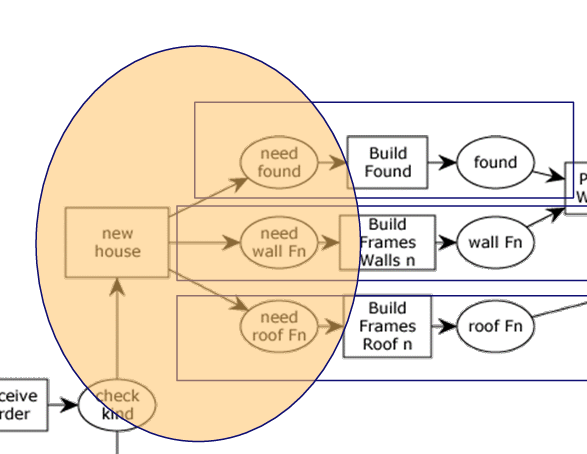
\includegraphics[scale=0.3]{capitolo 3/3-and-split.png}
        \end{subfigure}
        % Seconda immagine
        \begin{subfigure}{\textwidth}
            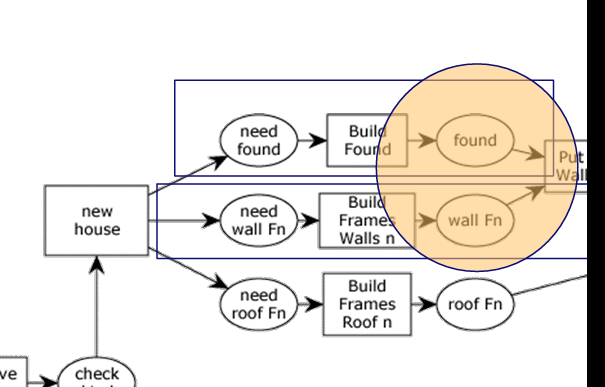
\includegraphics[scale=0.3]{capitolo 3/3-and-join.png}
        \end{subfigure}
        \caption{AND-split and AND-join: Concurrency Example}
    \end{figure}
    
    \subsection{XOR-split and XOR-join}
    An XOR-split occurs when a transition enables one of several possible output places, representing a decision point or choice. An XOR-join occurs when one of several input places enables a transition, resolving the choice.
    
    \begin{figure}[htbp][h]
        \centering
        % Prima immagine
        \begin{subfigure}{\textwidth}
            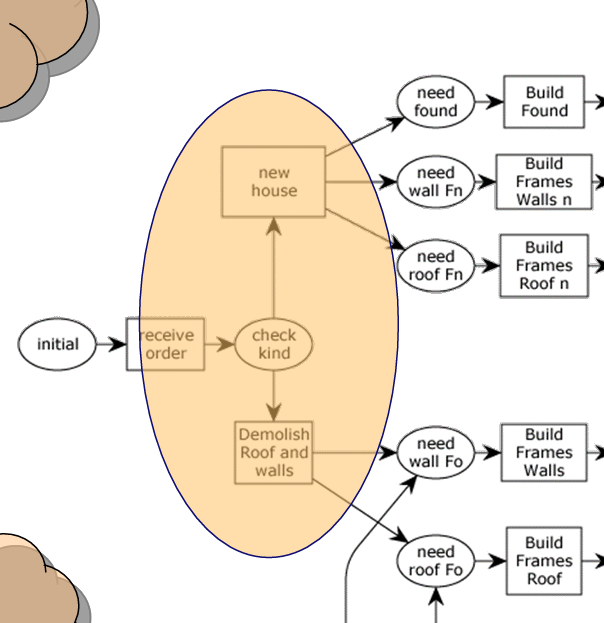
\includegraphics[scale=0.3]{capitolo 3/3-xor-split-choice.png}
        \end{subfigure}
        % Seconda immagine
        \begin{subfigure}{\textwidth}
            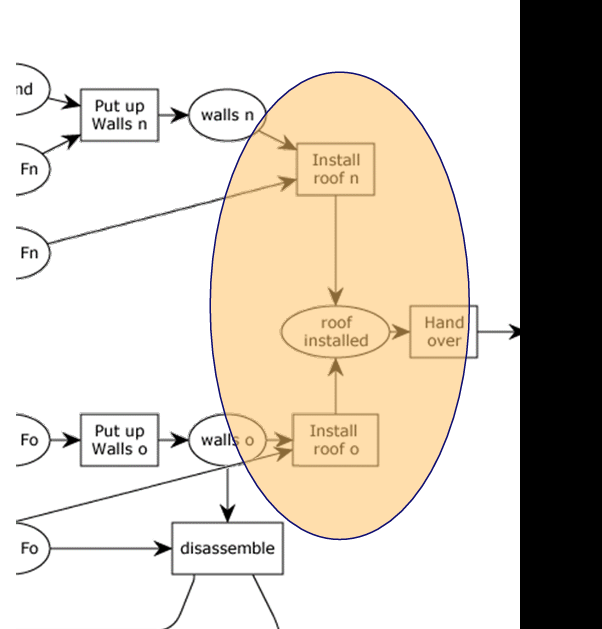
\includegraphics[scale=0.3]{capitolo 3/3-xor-join-choice.png}
        \end{subfigure}
        \caption{XOR-split and XOR-join: Choice Example}
    \end{figure}
    
    \subsection{Iteration}
    Iteration is modeled when a transition fires and produces tokens that eventually loop back into one of its input places, representing repetition or looping behavior.
    
    \begin{figure}[htbp][h]
        \centering
        % Prima immagine
        \begin{subfigure}{\textwidth}
            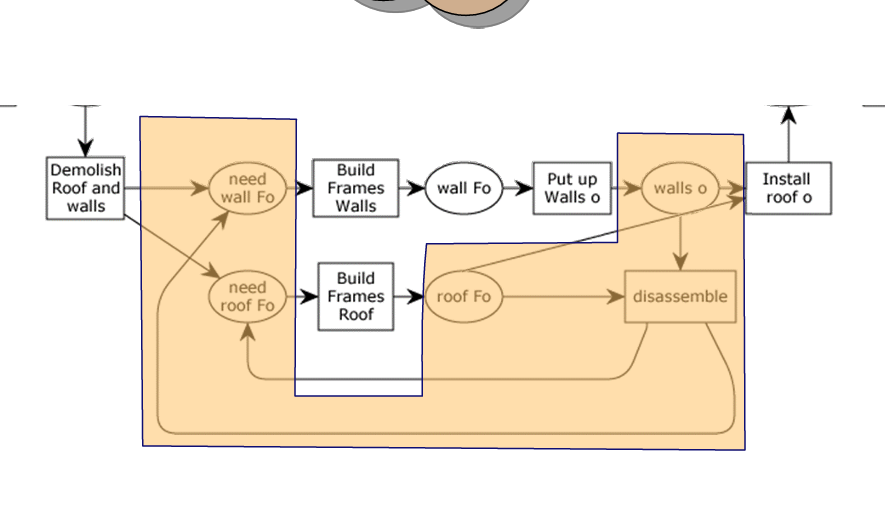
\includegraphics[scale=0.3]{capitolo 3/3-loop-iteration.png}
        \end{subfigure}
        % Seconda immagine
        \begin{subfigure}{\textwidth}
            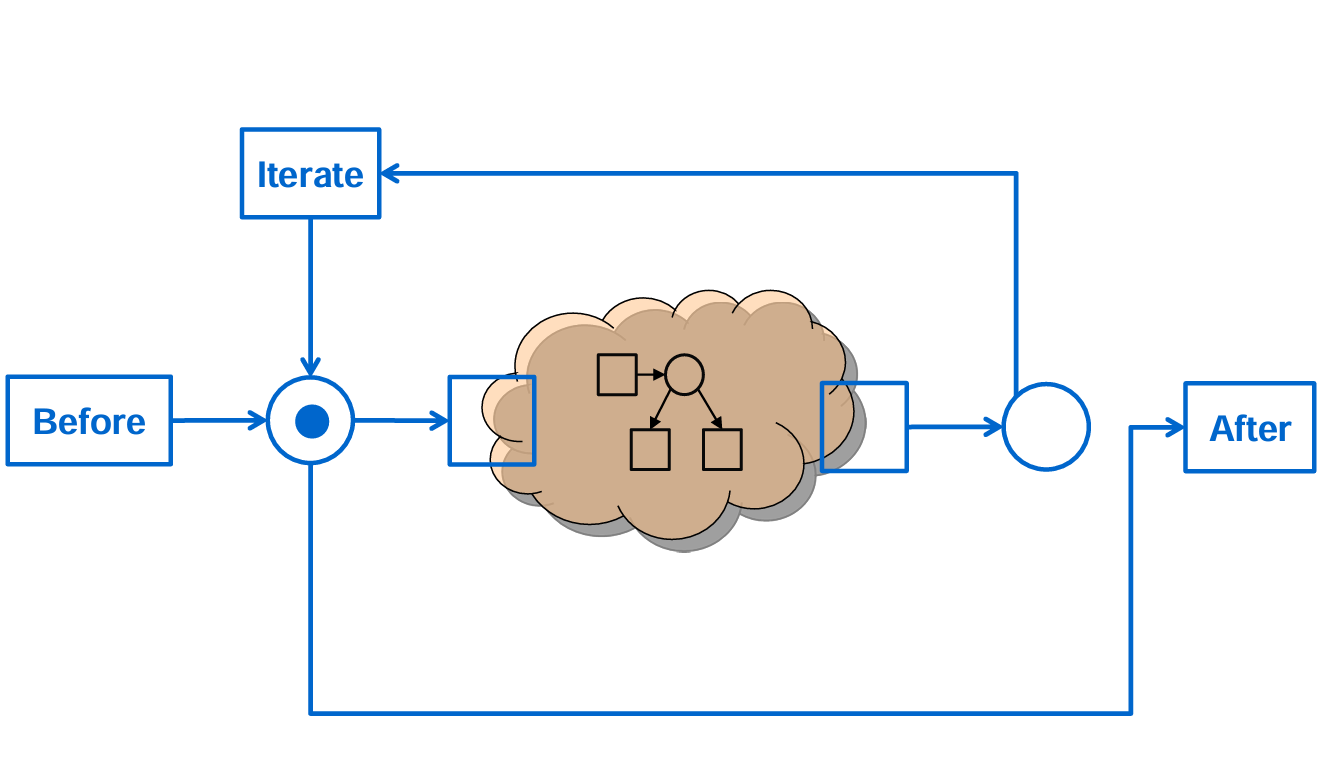
\includegraphics[scale=0.3]{capitolo 3/3-loop-iteration-0.png}
        \end{subfigure}
        \caption{Iteration Example}
    \end{figure}
    
    \section{Multi-token Arcs}
    
    In Petri nets, it is possible to have \textbf{multi-token arcs}, which either consume or produce more than one token at a time. These are represented by the following notation:
    
    \begin{figure}[h]
        \centering
        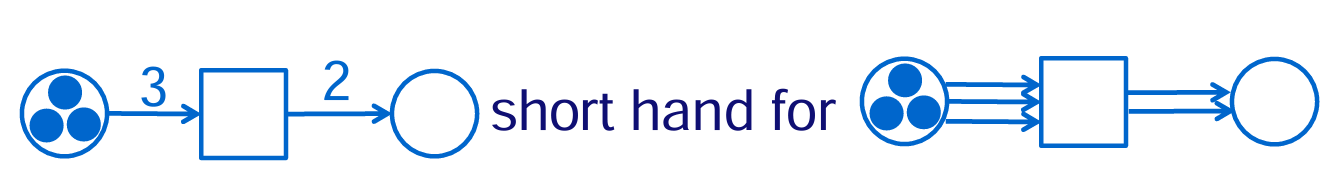
\includegraphics[scale=0.3]{capitolo 3/3-multiplearcs.png}
        % Insert multi-token arc example here
        \caption{Multi-token Arc Notation}
    \end{figure}
    
    \section{Formal Introduction to Petri Nets}
    
    
    A Petri net is a mathematical model used to represent distributed systems and processes, particularly useful in the analysis of systems with concurrency and synchronization. Formally, a Petri net is defined as a tuple \(PN = (P, T, F)\), where:
    
    \begin{itemize}
        \item \(P\) is a finite set of \textbf{places}.
        \item \(T\) is a finite set of \textbf{transitions}.
        \item \(F \subseteq (P \times T) \cup (T \times P)\) is the \textbf{flow relation}, defining directed arcs between places and transitions.
    \end{itemize}
    
    An example of a simple Petri net structure can be visualized with a place \(p_1\), a transition \(t\), and a place \(p_2\), where tokens move from \(p_1\) through \(t\) to \(p_2\):
    \[
    P = \{p_1, p_2\}, \quad T = \{t\}, \quad F = \{(p_1, t), (t, p_2)\}
    \]
    
    \subsection{Preset and Postset of a Transition}
    
    The preset and postset of a transition define its input and output places:
    \begin{itemize}
        \item The \textbf{preset} of a transition \(t\), denoted as \(\bullet t\), is the set of input places: 
        \[
        \bullet t = \{ p \mid (p, t) \in F \}
        \]
        \item The \textbf{postset} of a transition \(t\), denoted as \(t \bullet\), is the set of output places: 
        \[
        t \bullet = \{ p \mid (t, p) \in F \}
        \]
    \end{itemize}
    
    \subsection{Multisets}
    
    In Petri nets, markings are often represented as \textbf{multisets}, which differ from regular sets as they allow for multiple occurrences of the same element. The marking of a Petri net assigns a number of tokens to each place, and it can be represented either as a function or a vector. For example:
    \[
    m(p_1) = 1, \quad m(p_2) = 2, \quad m(p_3) = 0
    \]
    Alternatively, it can be written in vector notation:
    \[
    m = [p_1, 2 \cdot p_2]
    \]
    
    \subsection{Marking and Enabledness}
    
    A \textbf{marking} is a function \(m: P \to \mathbb{N}\) that assigns a non-negative number of tokens to each place. The marking defines the state of the Petri net. A transition \(t\) is \textbf{enabled} at a marking \(m\) if all of its input places have at least one token. Formally, \(t\) is enabled if:
    \[
    \forall p \in \bullet t, \ m(p) > 0
    \]
    
    \subsection{Transition Firing}
    
    When a transition \(t\) fires, it consumes one token from each of its input places and produces one token in each of its output places. The new marking \(m'\) after firing is given by:
    \[
    m'(p) = m(p) - w(p,t) + w(t,p) \quad \forall p \in P
    \]
    where \(w(p,t)\) is the weight of the arc from \(p\) to \(t\), and \(w(t,p)\) is the weight of the arc from \(t\) to \(p\).
    
    \subsection{Weight Function Definition}
    
    The \textbf{weight function} \(w: (P \times T) \cup (T \times P) \to \{0, 1\}\) assigns a value to each arc in the flow relation \(F\). For any pair \((x, y)\), where \(x\) is a place and \(y\) is a transition (or vice versa), the weight function is defined as follows:
    
    \[
    w((x, y)) = 
    \begin{cases}
    1, & \text{if} \ (x, y) \in F \\
    0, & \text{if} \ (x, y) \notin F
    \end{cases}
    \]
    This means an arc exists between \(x\) and \(y\) if and only if the weight is 1. Otherwise, the weight is 0.
    
    \subsection{Petri Net System}
    
    A \textbf{Petri net system} is defined as a Petri net with an initial marking. Formally, it is a tuple \(PN = (P, T, F, m_0)\), where \(m_0\) is the initial marking. For example:
    \[
    P = \{p_1, p_2, p_3\}, \quad T = \{t\}, \quad F = \{(p_1, t), (p_2, t), (t, p_3)\}
    \]
    \[
    m_0(p_1) = 1, \quad m_0(p_2) = 2, \quad m_0(p_3) = 0
    \]
    
    \subsection{Arc Multiplicities}
    
    Arc multiplicities represent how many tokens are consumed or produced during a transition firing. If a transition consumes or produces more than one token, the weight of the arc is indicated accordingly. For example, consuming two tokens from place \(p_1\) and producing three tokens in place \(p_2\) can be represented as:
    \[
    w(p_1, t) = 2, \quad w(t, p_2) = 3
    \]
    This means that when the transition \(t\) fires, it will consume 2 tokens from \(p_1\) and produce 3 tokens into \(p_2\).